The lack of quantitative knowledge about soot inception and surface growth pathways has hindered the development of accurate models for predicting soot mass and morphology. Uncertainties in the gas-phase chemistry of small and large intermediates can result in orders-of-magnitude differences in the predicted concentrations of PAHs~\citep{wang2023systematic}. These uncertainties are further amplified by inception models, making soot modeling even more challenging. As a result, the choice of reaction mechanism becomes a critical factor in soot simulations.

A series of simulations were performed using the CPR mode of omnisoot, excluding soot formation, to highlight the differences among six reaction mechanisms in describing gas-phase chemistry during the pyrolysis of a $10\%$ $\mathrm{CH_4}$-Ar mixture at $\mathrm{T_5}=$2200 K and $\mathrm{P_5}=$4.5 atm. The selected mechanisms include: ABF~\citep{appel2000kinetic}, Caltech~\citep{blanquart2009chemical}, KAUST~\citep{wang2013pah}, CRECK~\citep{saggese2015kinetic}, ITV~\citep{hellmuth2024role}, NUIG~\citep{zhu2023wide}. These mechanisms have been widely used for flame and reactor modeling. The last three have been actively developed and tested in recent years. 

The comparison focuses on the predicted Carbon Mass Fraction (CMF) of species involved in soot formation. Here, CMF is defined as the mass of carbon in a given species normalized by the total carbon mass in the gas mixture, which remains constant in the absence of soot formation. Initially, the CMF of methane is equal to 1, indicating that all carbon is stored in $\mathrm{CH_4}$ at $t = 0$ in the studied shock tube. %It should be noted that the CRECK mechanism used in this work does not include ``BIN" species, except for BIN1.


Figure~\ref{fig:CH4_C2H4_A2R5_chem} shows the variability in the predicted CMF of $\mathrm{CH_4}$, $\mathrm{C_2H_2}$, and A2R5 across different reaction mechanisms. The CMF of $\mathrm{CH_4}$ serves as a useful indicator of carbon flux from the fuel to intermediate species. $\mathrm{C_2H_2}$ is the most abundant hydrocarbon during pyrolysis and plays a key role in the HACA mechanism for PAH growth beyond benzene, as well as in surface growth of soot. A2R5 has been identified as important for soot inception, due to its low-aromaticity free edge, which readily reacts with $\sigma$-radicals and, if partially hydrogenated, can form localized $\pi$-radicals that enable combined covalent/stacked complex formation~\citep{martin2019reactivity}.

As shown in the inset of Figure~\ref{fig:CH4_C2H4_A2R5_chem}a, the CRECK mechanism predicts the highest $\mathrm{CH_4}$ conversion up to 1 ms, but this trend reverses at longer residence times, where KAUST predicts the lowest CMF. ABF and NUIG underpredict the methane conversion rate by nearly 10\% of the initial carbon compared to the other mechanisms. As expected, the majority (40–60\%) of the initial carbon is converted to $\mathrm{C_2H_2}$ by the end of the simulation. In the inset of Figure~\ref{fig:CH4_C2H4_A2R5_chem}b, all mechanisms direct more carbon toward $\mathrm{C_2H_2}$ by 5 ms. CRECK predicts the highest $\mathrm{C_2H_2}$ CMF up to 1 ms, after which NUIG gives the largest $\mathrm{C_2H_2}$ CMF. This is attributed to NUIG’s lack of aromatic and large hydrocarbon species, so it does not account for the conversion of $\mathrm{C_2H_2}$ to PAHs.

The relative difference between the mechanisms is most pronounced for A2R5, spanning over an order of magnitude between ABF and Caltech. This aligns with previous findings that the uncertainty in the predicted concentration of gas-phase species increases with molecular size~\cite{wang2023systematic}. Since soot inception is described as the dimerization of PAHs, such discrepancies are amplified resulting in a one-order-of-magnitude variation in monomer concentration can lead to a two-order-of-magnitude difference in dimer formation.
 
\begin{figure}[H]
	\centering
	\begin{subfigure}[t]{0.31\textwidth}
		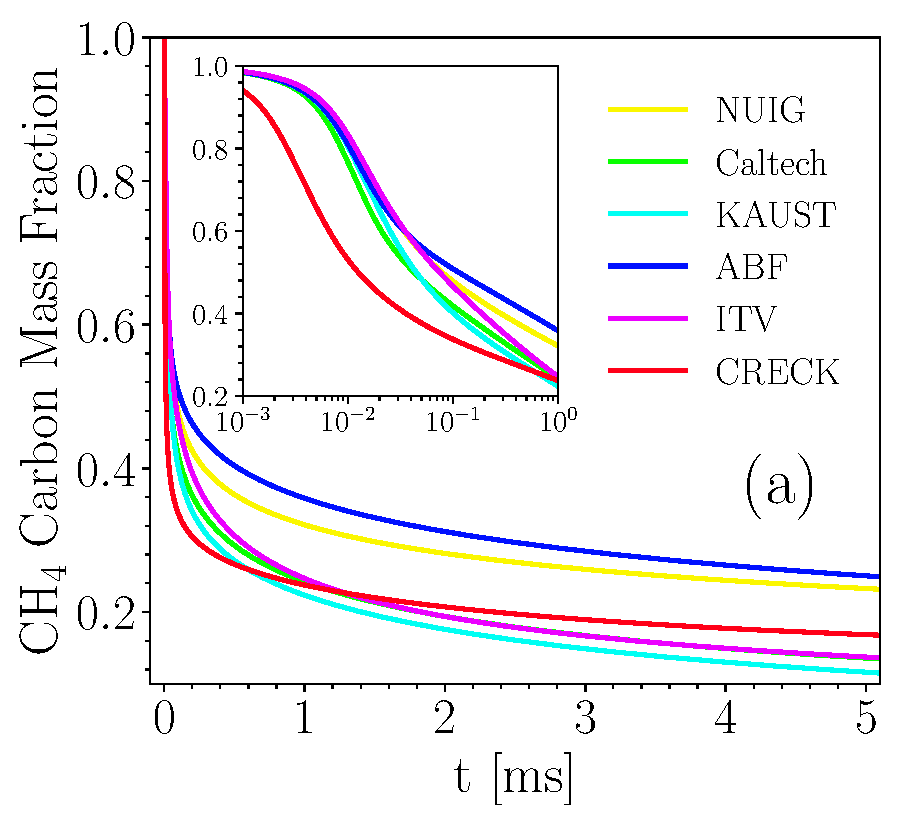
\includegraphics[width=1\textwidth]{Figures/Results/chemistry/CH4.pdf}
	\end{subfigure}
	\begin{subfigure}[t]{0.31\textwidth}
		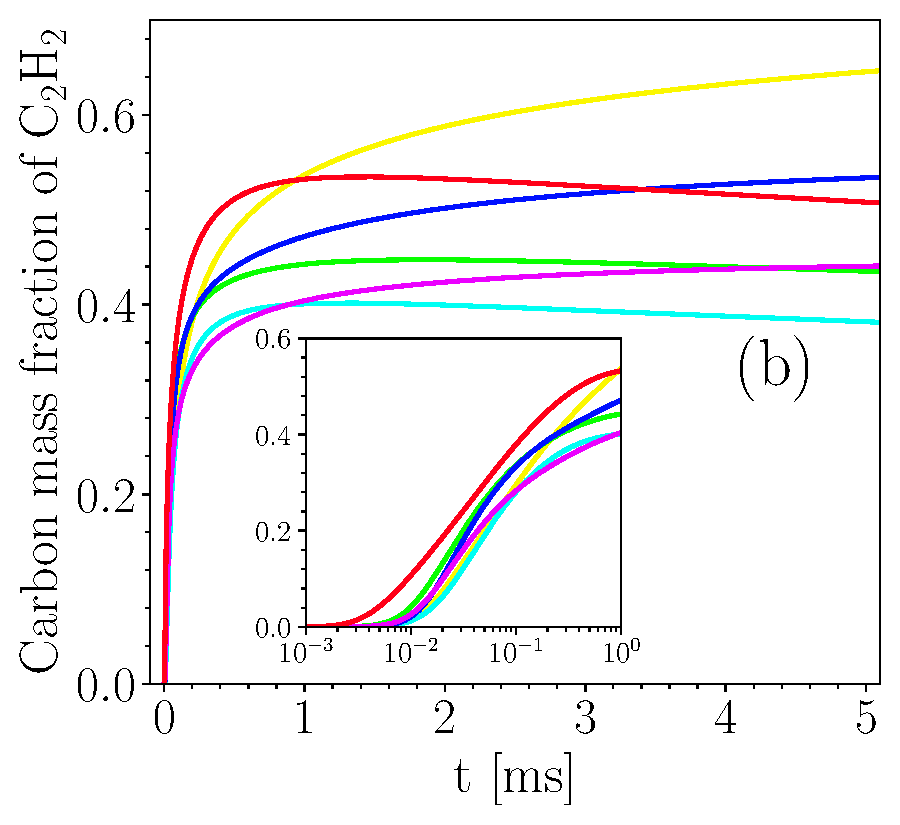
\includegraphics[width=1\textwidth]{Figures/Results/chemistry/C2H2.pdf}
	\end{subfigure}
	\begin{subfigure}[t]{0.31\textwidth}
		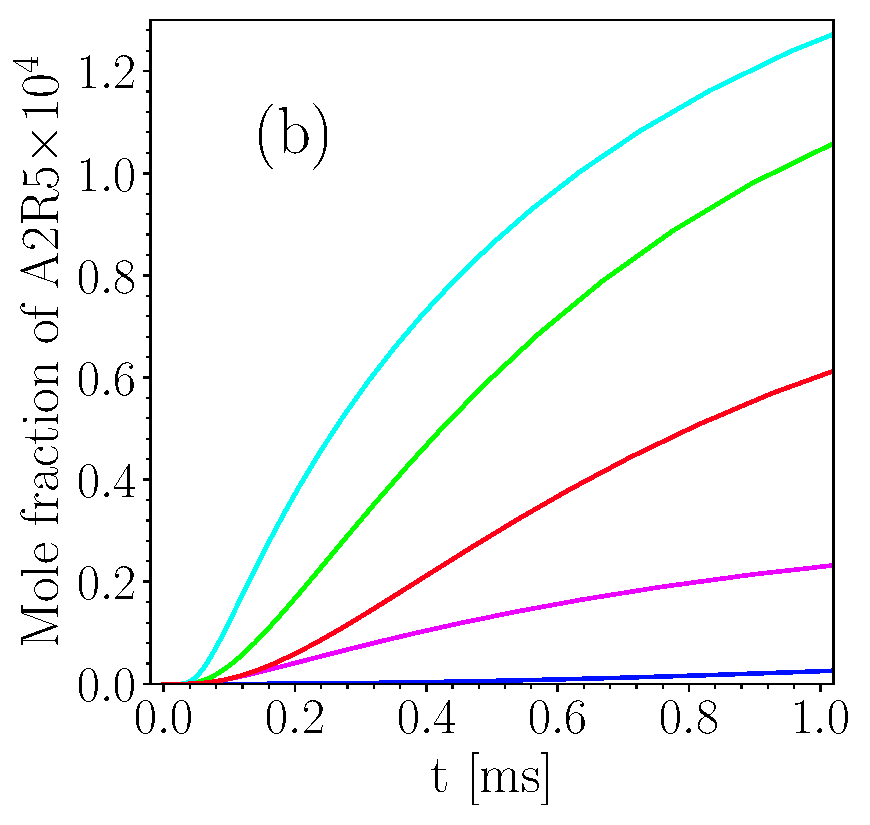
\includegraphics[width=1\textwidth]{Figures/Results/chemistry/A2R5.pdf}
	\end{subfigure}
	\caption{The carbon mass fraction of $\mathrm{CH_4}$ (a), $\mathrm{C_2H_2}$ (b), and A2R5 (c) during pyrolysis of 10\%~$\mathrm{CH_4}$-Ar predicted using different reaction mechanisms. The insets provide a zoomed-in view of the early-time behavior}
	\label{fig:CH4_C2H4_A2R5_chem} 
\end{figure}

Omnisoot supports all standard reaction mechanisms through Cantera. However, soot simulations in this study were conducted using Caltech and KAUST mechanisms, as both include the designated soot precursors and yield high carbon fluxes to PAHs, resulting in soot yields and volume fractions that closely match experimental measurements. Although the ITV mechanism also meets these criteria, its large size (759 species and 7582 reactions) significantly increases the computational cost of parametric studies and simulations.

%
%\begin{figure}[H]
%	\centering
%	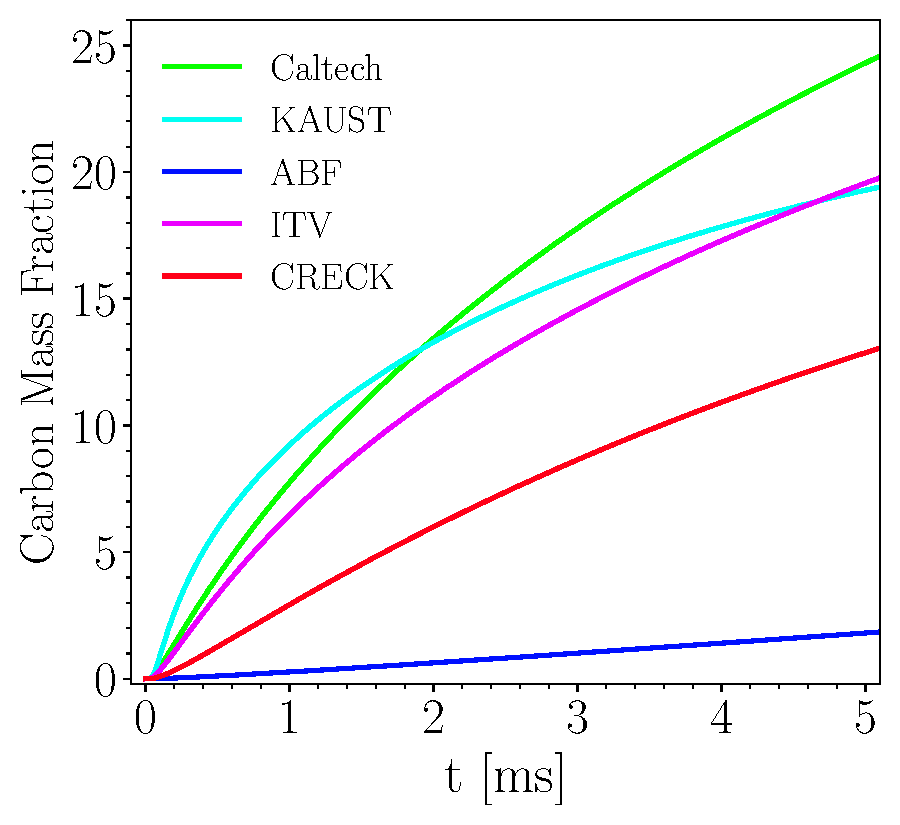
\includegraphics[width=0.32\textwidth]{Figures/Results/chemistry/med_hydrocarbons.pdf}
%	\caption{The carbon mass fraction of $\mathrm{C_{10}}$ to  $\mathrm{C_{18}}$ during pyrolysis of 10\%~$\mathrm{CH_4}$-Ar predicted using different reaction mechanisms}
%	\label{fig:PAHs_chem} 
%\end{figure}